\documentclass[10pt, titlepage, oneside, a4paper]{article}
\usepackage[style=authoryear]{biblatex}
\addbibresource{bibliography.bib}

\usepackage[T1]{fontenc}
\usepackage[titletoc]{appendix}
\usepackage[utf8]{inputenc}
\usepackage{amssymb, graphicx, fancyhdr}
\usepackage{amsmath}
\usepackage{amsthm,algorithm,algorithmic,yhmath,enumitem,lscape}
\usepackage{float}
\usepackage{hyperref, url}
\usepackage{minted}
\newmintinline{c}{}
\addtolength{\textheight}{20mm}
\addtolength{\voffset}{-5mm}
\def\inst{Computing Science}
\def\course{5DV243 Artificial Intelligence}
\def\title{Assignment 1 --- Othello}

%%%%%%%%%%%%%%%%%%%%%%%%%%%
\def\names{Sienichev Matvey, Afrasah Benjamin Arko} 
\def\csusernames{ens25msv, mai25bah}
\def\graders{Filip Naudot, Timotheus Kampik, Igor Ryazanov}
%%%%%%%%%%%%%%%%%%%%%%%%%%%%


\def\mfullpath{\raisebox{1pt}{$\scriptstyle \sim$}\musername/\path}
\def\nfullpath{\raisebox{1pt}{$\scriptstyle \sim$}\nusername/\path}
\newcommand{\R}{\mathbb{R}}
\newcommand{\N}{\mathbb{N}}
\newcommand{\Rnn}{\mathbb{R}^{n \times n}}
\newcommand{\bes}{\begin{equation*}}
\newcommand{\ees}{\end{equation*}}
\newcommand{\be}{\begin{equation}}
\newcommand{\ee}{\end{equation}}
\newcommand{\bms}{\begin{multline*}}
\newcommand{\emults}{\end{multline*}}
\newcommand{\bbm}{\begin{bmatrix}}
\newcommand{\ebm}{\end{bmatrix}}
\newcommand{\eps}{\epsilon}
\newcommand{\fl}{\text{fl}}
\newcommand{\Lp}{{L^p}}
\newcommand{\Ker}{\text{Ker}\,}
\newcommand{\loc}{{\text{loc}}}
\newcommand{\ccinf}{C_c^\infty}
\newcommand{\supp}{\text{supp}}
\newcommand{\dist}{\text{dist}}

\begin{document}
	\begin{titlepage}
		\thispagestyle{empty}
		\begin{large}
			\begin{tabular}{@{}p{\textwidth}@{}}
				\textbf{\hfill \today} \\
				
				%\textbf{\typeofdoc} \\
			\end{tabular}
		\end{large}
		\vspace{25mm}
		\begin{center}
			%\LARGE{\pretitle} \\
			\huge{\textbf{\course}}\\
			\vspace{10mm}
			\LARGE{\title} \\
			\vspace{15mm}
            \LARGE{version 1.0} \\
            \vspace{10mm}
			\begin{large}
				\begin{tabular}{ll}
					\textbf{Names} & \names \\
					\textbf{CS usernames} & \csusernames 
				\end{tabular}
			\end{large}
			\vfill
            \vfill
			\large{\textbf{Graders}}\\
			\mbox{\large{\graders}}
		\end{center}
	\end{titlepage}
    
    % fixar sidfot
	%\lfoot{\footnotesize{\name, \username}}
	\rfoot{\footnotesize{\today}}
	\lhead{\sc\footnotesize\title}
	\rhead{\nouppercase{\sc\footnotesize\leftmark}}
	\pagestyle{fancy}
	\renewcommand{\headrulewidth}{0.2pt}
	\renewcommand{\footrulewidth}{0.2pt}

	% skapar innehållsförteckning.
	% Tänk på att köra latex 2ggr för att uppdatera allt
	%\pagenumbering{roman}
	%\tableofcontents
	% och lägger in en sidbrytning
	%\newpage

	\pagenumbering{arabic}

	% i Sverige har vi normalt inget indrag vid nytt stycke
	\setlength{\parindent}{0pt}
	% men däremot lite mellanrum
	\setlength{\parskip}{10pt}

\addtocounter{section}{0}
%\section{Changes}
%If this is a resubmission, include a list of changes %with respect to
%the previous submission.

\section{Introduction}
\label{sec:intro}
% Also possible to use \input{intro.tex} to break down the report into one file per section
Robots have been beating humans in more and more domains every day. This is also the case for Othello, a strategic turn based board game. As such, to fight fire with fire, we attempted to create an Othello game engine capable of outperforming a simple fixed depth search of 7, piece count based game engine. 
We used python for this task, which can be around 10 to 100 times slower than a compiled language, because of that we had to use a couple of tricks to outcompete a Java written engine within reasonable compute times, ideally in less than 3 seconds per move, both as black and as white player. To achieve these times while still keeping a sufficient compute depth our engine implements alpha beta search algorithm that offers a substantial speed up compared to a min/max algorithm. While that allows us to go to depths greater than 7 in the early game, as well as in the endgame, during midgame the branching factor is too high to allow it to compute in under 3 seconds, that's why our algorithm uses an iterative deepening approach, starting at depth 3 and evaluating iteratively deeper and deeper as long as the maximum time for the move hasn't been exceeded. Unfortunately, that means that for some moves the decisions are made having less information about all the possible states of the board than the adversary. To make up for the short-sightedness of our algorithm we implemented some clever heuristics that mimic human long term strategy thinking to evaluate the score of every position. 
Firstly we will discuss the technical details of our implementation\ref{sec:methods}, after that we will give results \ref{sec:results} and finally analyze them and discuss possible improvements \ref{sec:discussion}



\subsection{Reproducibility and Environment}
Our implementation uses Python 3.13.5 on macOS (Darwin 25.0.0, ARM64 architecture). The engine runs without any special compiler flags since Python is an interpreted language.

To run our engine with the provided \texttt{othello.sh}:
\begin{minted}{bash}
./othello.sh <position_string> <time_limit_seconds> <do_compile>
# Example:
./othello.sh WEEEEEEEEEEEEEEEEEEEEEEEEEEEEEEEEEEEEEEEEEEEEEEEEEEEEEEEEEEEEEEEE 5 0
\end{minted}

\section{Methods}
\label{sec:methods}


\subsection{Position Representation}
Currently a position is being stored as an array of arrays 10 by 10 of 8 bit characters, with the borders being empty, so effectively only a 64 square zone is used to play. 
Every square in Othello game can be either occupied by a black disc, a white disc or empty. These 3 states are represented by storing a 'W', a 'B' or an 'E' characters in the array representing the board.
For example to put a white disc on a first row of a second column, we do it as shown in Figure~\ref{fig:board_representation}
\begin{figure}[h]
    \centering
    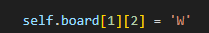
\includegraphics[width=0.6\textwidth]{img/board_representation}
    \caption{Board representation}
    \label{fig:board_representation}
\end{figure}
This is the easiest way to do it because it is a straightforward implementation of a real world Othello board as we humans perceive it. 

\subsection{Search Algorithm: Alpha--Beta}

Our implementation uses standard minimax with alpha-beta pruning. The \texttt{AlphaBeta} class provides:
\begin{minted}{python}
def evaluate(self, othello_position: OthelloPosition) -> OthelloAction
def max_value(self, pos: OthelloPosition, alpha: float, 
              beta: float, depth: int) -> OthelloAction
def min_value(self, pos: OthelloPosition, alpha: float, 
              beta: float, depth: int) -> OthelloAction
\end{minted}

White is MAX (the player with the highest score), and Black is MIN (the player with the lowest score) however evaluator maintains consistent perspective using \texttt{playing\_white}. The search terminates at \texttt{depth == 0} or when no legal moves exist, then we evaluate the positions with the heuristic.

MAX nodes update \texttt{alpha = max(alpha, best\_value)}, MIN nodes update \texttt{beta = min(beta, best\_value)}. Pruning occurs when \texttt{alpha >= beta}.

We implemented a move ordering enhancement to prioritize searching for promising moves to improve the pruning efficiency \textcite{russell2020artificial}. 

\texttt{Corners (1000) > Edges (100) > Center (10) > Regular (1) > C-squares (-500) > X-squares (-1000) > Pass (-inf)}

\subsection{Iterative Deepening \& Time Control}
Unlike the naive player which searches at a fixed depth of 7, we implemented 
\textit{Iterative Deepening Search (IDS)} with depth increments of 1. 
This gives us the best move from the deepest search we managed to complete 
until we ran out of time.

Our time control is cooperative. We check the clock during a search and throw 
a \texttt{StopSignal} exception when time runs out. The exception is caught by 
the main loop and returns the best move so far. For each iteration, we compute 
the remaining time and pass it to our \texttt{AlphaBeta} algorithm, which checks 
at every 1000th node if we have enough time.

In order not to run out of time, we utilize 90\% of the allocated time. 
This gives us a small buffer for evaluation overhead while maximizing our 
search depth.

One main advantage of iterative deepening is that even if we get cut off 
mid-search, we still have a complete result from previous depths.

% Explain how you replaced fixed-depth with Iterative Deepening Search (IDS) and describe how you enforce your time budget. 

% If your search is \emph{cooperative}, describe where you check time (e.g., on node entry, inside move loops), how you signal timeout (e.g. return flag or exception), and how the top-level search preserves the best move from the last completed depth.

% Optionally discuss thread/process-based control (e.g., main thread owns the clock; worker thread does search and checks a stop flag).
% If you used a hard cutoff (separate process), briefly explain the serialization of moves.

\subsection{Heuristics}


For our heuristics, our evaluation function is a significant development of the \texttt{CountingEvaluator} which just counts pieces. We developed a 10 feature heuristic system that captures the strategic features of Othello gameplay through careful analysis of established game theory and empirical testing.

\subsubsection{Evolution from CountingEvaluator}
The \texttt{CountingEvaluator} gave a basic evaluation by just counting the difference between the discs of the current player and the opponent:
\begin{equation}
\text{Score} = \text{my\_pieces} - \text{opp\_pieces}
\end{equation}

This approach only has merit in the last phase of the game when mobility is limited and does not capture the strategic complexity of Othello. Our enhanced evaluation addresses the limitations of piece counting through a comprehensive analysis of features that affect gameplay.

\subsubsection{Feature Engineering and Strategic Analysis}

Our evaluation uses a weighted linear combination \cite{russell2020artificial} with 10 strategic features:
\begin{equation}
\text{Score} = \sum_{i=1}^{10} w_i \cdot f_i
\end{equation}
Where $w_i$ are the optimized weights and $f_i$ are the extracted features. The features are calculated from the perspective of the starting player.

We improved our weights by focusing on stability, mobility and corner control, and penalizing dangerous positions through gameplay analysis and testing with the naive \textcite{brianothello2005}.
Overall, we managed to capture the limitations of the naive piece counting player.

\begin{table}[H]
\centering
\footnotesize
\begin{tabular}{|l|l|c|c|}
\hline
\textbf{Feature} & \textbf{Formula} & \textbf{Weight} & \textbf{Description} \\
\hline
\multicolumn{4}{|c|}{\textbf{Stability Control}} \\
\hline
Corner Control & $my\_corners - opp\_corners$ & 600.0 & Corner occupation \\
\hline
Edge Control & $my\_edges - opp\_edges$ & 70.0 & Edge position control \\
\hline
Stability & $my\_stability - opp\_stability$ & 90.0 & Unflippable discs \\
\hline
\multicolumn{4}{|c|}{\textbf{Risk Avoidance}} \\
\hline
X-Squares & $my\_x\_squares - opp\_x\_squares$ & -50.0 & Dangerous corner-adjacent \\
\hline
C-Squares & $my\_c\_squares - opp\_c\_squares$ & -5.0 & Risky corner-adjacent \\
\hline
Frontier Discs & $my\_frontier - opp\_frontier$ & -10.0 & Vulnerable flippable pieces \\
\hline
\multicolumn{4}{|c|}{\textbf{Mobility Control}} \\
\hline
Mobility & $my\_mobility - opp\_mobility$ & 100.0 & Legal moves available \\
\hline
Potential Mobility & $my\_potential - opp\_potential$ & 6.0 & Future move opportunities \\
\hline
\multicolumn{4}{|c|}{\textbf{Piece Difference}} \\
\hline
Piece Difference & $my\_pieces - opp\_pieces$ & 100.0 & Disc count advantage \\
\hline
\multicolumn{4}{|c|}{\textbf{Game Phase Adaptation}} \\
\hline
Parity Score & 1 or 0 & 18.0 & Move timing control \\
\hline
\end{tabular}
\caption{Complete Heuristic Feature Set with Formulas and Weights}
\end{table}


\setcounter{secnumdepth}{4}
\subsubsection{Stability Control}

\vspace{0.5em}

\textbf{Corners} (Weight: 600.0) are the most strategically important positions because they can never be flipped once captured\cite{brianothello2005}.  They serve as a foundation for building more stable discs. They make it possible to build more stable discs and often decide the outcome of the game\cite{brianothello2005}.

\textbf{Edge positions} (Weight: 70) gives strategic advantages for making paths to corners and making it harder for your opponent to move.  But they need to be balanced carefully, because taking the edge too soon can make you weak in the early game\cite{brianothello2005}.  The medium weight shows how important edge control is, which gets more important as the game goes on.

\textbf{Stable discs} (Weight: 90.0) are those that no opponent move can flip.  Our stability analysis uses a simple heuristic method to estimate stability, taking into account the following: (1) corners are always stable and worth 3x as much, (2) edges are somewhat stable and worth 1x as much, and (3) interior pieces are assumed to be neutral and not counted.  This method of estimating disc stability gives a good idea of how stable it is without the need for complicated calculations \cite{othello-heuristics-analysis}. 



\subsubsection{Risk Avoidance}

\vspace{0.5em}

\textbf{X-Squares} (Weight: -50.0) are the diagonal squares next to the corners.  These positions are very risky because they often let the other player capture the corner \cite{brianothello2005}.  The strong negative weight shows that the tactical rule is to avoid X-square occupation unless it is absolutely necessary.

\textbf{C-Squares} (Weight: -5.0) are squares that are right next to corners.  C-squares are less dangerous than X-squares, but they can also lead to corner loss through tactical sequences \cite{brianothello2005}.  
The moderate negative weight reflects how occupying a C-square might be okay in some situations.

\textbf{Frontier Discs} (Weight: -10.0) are those next to empty squares. We negatively weight them because having more frontiers reduces your stability and increases your opponent's mobility\cite{brianothello2005}.

\subsubsection{Mobility Control}

\vspace{0.5em}

\textbf{Mobility} (Weight: 100.0) is the number of legal moves a player can make.  High mobility gives players the freedom to make strategic and tactical choices, which lets them avoid being forced to move to bad positions \cite{cohen2020learning}.

\textbf{Potential Mobility} (Weight: 6.0) counts empty squares next to opponent pieces, which show where they could move in the future.  A higher opponent potential mobility is bad because it means they have more strategic options\cite{buro1995othello}.  This feature helps you think about long-term tactical options that go beyond just legal moves right now.

\subsubsection{Piece Difference}

\vspace{0.5em}

\textbf{Piece Difference} (Weight: 100) plays a significant role in the last stages of the game when mobility is limited \cite{othello-heuristics-analysis}.

\subsubsection{Game Phase Adaptation}

\vspace{0.5em}
\textbf{Parity Score} (Weight: 18.0) determines tempo advantages based on remaining moves and current disc count. If remaining moves are even, the player ahead in discs has advantage. If remaining moves are odd, the player behind in discs benefits from the extra move \cite{brianothello2005}. This binary feature (0 or 1) helps evaluate endgame positioning and move timing advantages.


\subsection{makeMove() / Action Generation}
A move is represented by 2 integers, representing the placement of a disc on a board as well as a boolean that is set to True if the move is a pass move. Because the move is applied to an instance of the Othello position the color of the disc will be placed according to the instances attribute \textit{maxPlayer}
In case of a pass move the current player will be changed and a resulting Othello position will be returned. Otherwise the function will loop though all of the 8 possible directions and for every direction if the capture is possible, it will flip the discs until the function finds one of our own discs. The code for this function is shown below.

\begin{minted}[linenos=true=autogobble]{python}
#makeMove() loop
for dir in self.DIRS:
    capture = self.__captures_in_direction(action.row, action.col, dir[0], dir[1])
    if(capture == True):
        i = 1
        while(self.__is_opp_coin(action.row+dir[0]*i, action.col+dir[1]*i)):
        self.board[action.row+dir[0]*i, action.col+dir[1]*i] = current_player
        i = i+1
\end{minted}



\section{Results}
\label{sec:results}
We tested our engine against the naive engine (fixed depth 7, piece counting) across time limits 2s-10s for both counting and heuristic evaluators, playing as both White and Black. Metrics include win/loss, final scores, and average search depth during mobility phase (moves 10-40). All games were deterministic with no randomness.


\subsection{Test runs}
\label{sec:testruns}

\begin{table}[H]
    \centering
    \caption{Performance using counting evaluator (2s-10s)}
    \begin{tabular}{ccccc}
    \hline
    \textbf{Color} & \textbf{Time limit} & \textbf{Result} & \textbf{Average depth} & \textbf{Depth range} \\
    \hline
    White & 2s & Black won with 38 & 6 & 5-7\\
    Black & 2s & Black won with 42 & 5 & 5-6\\
    White & 3s & Black won with 46 & 6 & 5-8\\
    Black & 3s & White won with 12 & 5 & 5-7\\
    White & 4s & Black won with 30 & 7 & 6-9\\
    Black & 4s & White won with 26 & 5 & 5-7\\
    White & 5s & White won with 38 & 6 & 5-7\\
    Black & 5s & White won with 40 & 6 & 6-7\\
    White & 6s & Black won with 0 & 6 & 6-8\\
    Black & 6s & Black won with 8 & 6 & 6-7\\
    White & 7s & White won with 10 & 6 & 6-7\\
    Black & 7s & Black won with 22 & 6 & 6-7\\
    White & 8s & White won with 4 & 6 & 6-7\\
    Black & 8s & Black won with 12 & 6 & 6-8\\
    White & 9s & White won with 24 & 6 & 6-8\\
    Black & 9s & White won with 4 & 6 & 6-7\\
    White & 10s & White won with 22 & 6 & 6-8\\
    Black & 10s & Black won with 0 & 6 & 6-7\\
    \hline
    \end{tabular}    
    \label{tab:counting-results}
\end{table}

\begin{table}[H]
    \centering
    \caption{Performance using heuristic evaluator (2s-10s)}
    \begin{tabular}{ccccc}
    \hline
    \textbf{Color} & \textbf{Time limit} & \textbf{Result} & \textbf{Average depth} & \textbf{Depth range} \\
    \hline
    White & 2s & White won with 44 & 4 & 4-5\\ 
    Black & 2s & Black won with 60 & 4 & 4-6\\
    White & 3s & White won with 64 & 5 & 4-6\\
    Black & 3s & Black won with 40 & 5 & 4-6\\
    White & 4s & White won with 56 & 5 & 5-6\\
    Black & 4s & Black won with 62 & 5 & 5-6\\
    White & 5s & White won with 64 & 5 & 5-6\\
    Black & 5s & Black won with 63 & 5 & 5-6\\
    White & 6s & White won with 64 & 5 & 5-6\\
    Black & 6s & Black won with 63 & 5 & 5-7\\
    White & 7s & White won with 64 & 5 & 5-6\\
    Black & 7s & Black won with 63 & 5 & 5-7\\
    White & 8s & White won with 64 & 5 & 5-6\\
    Black & 8s & Black won with 63 & 5 & 5-7\\
    White & 9s & White won with 64 & 6 & 6-6\\
    Black & 9s & Black won with 52 & 5 & 4-7\\
    White & 10s & White won with 64 & 6 & 6-7\\
    Black & 10s & Black won with 52 & 5 & 4-8\\
    \hline
    \end{tabular}    
    \label{tab:heuristic-results}
\end{table}


\subsubsection{Results Analysis}
The counting evaluator achieved mixed results (54\% White, 45\% Black win rates) with inconsistent performance across 2s-10s time limits. The simple piece-counting evaluation was insufficient against the naive engine.

Our heuristic evaluator achieved perfect 100\% win rates as both colors across all time limits (2s-10s), with multiple 64-point victories as White and strong Black performances (52-63 points). Average search depth remained at 5-6, demonstrating that superior evaluation quality compensated for reduced search depth.

Key strategic features - corner control and mobility provided significant advantages. Move ordering improved alpha-beta pruning efficiency. No time overruns occurred with iterative deepening using 90\% time utilization.

\textbf{Assignment Requirement}: Our heuristic evaluator consistently beat the naive engine under 2-10 seconds as both colors, proving that strategic evaluation features can overcome deeper fixed-depth search.

\section{Discussion}
\label{sec:discussion}
Representing the board as an array of arrays is easy to implement, however, it is not very efficient. Indeed, each character takes 1 byte of memory, so a full board takes 100 bytes. 
The deeper we go, the more positions we have to evaluate, for example for the depth of 7 with a random evaluation ordering, we can on average achieve a complexity of $O\big(b^{3d/4}\big)$ \textcite{alpha_beta_complexity} so with a branching factor of 10 the number of positions to evaluate would be 177 830, taking 100 bytes per position, the memory usage would be around 16 Megabytes, which is not that much and can fit in a cache of a modern CPU, however using the same calculation for a depth of 10 would yield 31 million positions to evaluate and would take 3GB in memory alone, that would not fit in a cache of any CPU, so frequent memory swaps will slow it down. 
A use of a bitboard would have allowed for a more efficient use of memory as it only requires two 64-bit integers to store a position (1 representing the black discs and the other white discs positions). It would have allowed to fit a whole position in only 2 bytes. So for the depth of 10, 31 millions positions would have used only 59MB, a much more memory efficient approach.
However, in python creating a class instance is memory intensive in itself, to have even better memory efficiency the better approach would have been to write the evaluator in an imperative low level programming language like C.
However even in python a use of bitboard would have allowed for a much more efficient computation, because some operations can be done only using one CPU instruction, such as for example instead of looping through the whole array to evaluate a position it could be done by applying a couple of masks to the integer representing disc positions.  


\section{Reflections}
\label{sec:reflections}

We first started by implementing the TODO sections of the provided code. We then wrote some unit tests to ensure that there were no bugs in our position representation and in the utility functions. To better understand the problem and establish a working baseline for improvement as well as validate the rest of our code, we first implemented the simple fixed-depth MinMax algorithm. We then implemented the full alpha beta search and iterative deepening. It was quite challenging to implement the Alpha Beta algorithm, so we both developed our solutions independently to be able to both understand it and avoid any bugs by comparing our solutions. It worked but seeing that our program was still not compliant with the time constraints that we had Benjamin improved the heuristic while Matvey was trying to implement the bitboard representation to improve performance, that was finally scrapped as it still had unresolved bugs by the time we had to turn our project in and was not necessary anymore as at that point the program was consistently winning as both black and white player thanks to the heuristic.   

\printbibliography

\end{document}